\chapter{Xây dựng và đánh giá mô hình}

\section{Thu thập và tiền xử lý dữ liệu}

Trong niên luận sử dụng bộ dữ liệu tiếng nói điều 
khiển của Google, bao gồm 85,511 tệp âm thanh 
tiếng nói với 35 từ khác nhau, mỗi tệp kéo dài trong một giây. Tập dữ liệu đã được chia thành các danh mục khác nhau như số, động vật, chỉ đường hoặc tên người. Bằng cách đó, hệ thống có thể được huấn 
luyện với các mục đích cụ thể hơn. Tập dữ liệu này 
được chia thành ba phần, bao gồm 80\% tập huấn 
luyện, 10\% tập đánh giá và 10\% thử nghiệm.
Từ khóa: Lớp từ khóa được gắn nhãn riêng, 
chứa một tập hợp các từ có liên quan. Trong bài báo
này các từ như "up", "down", "left", "right", "zero", "one", "two",... được chọn để thực hiện nhận dạng tiếng nói.
\begin{figure}
    \centering
    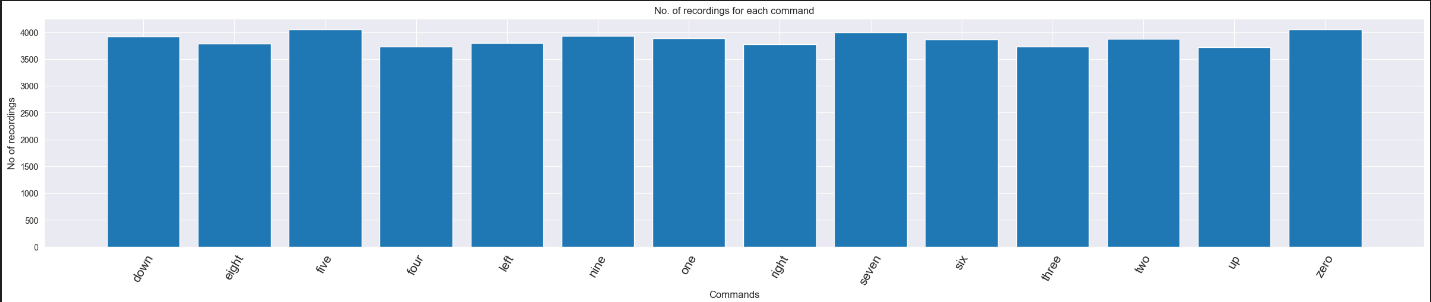
\includegraphics[width=0.5\linewidth]{images/data.png}
    \caption{Enter Caption}
    \label{fig:enter-label}
\end{figure}

\begin{figure}
    \centering
    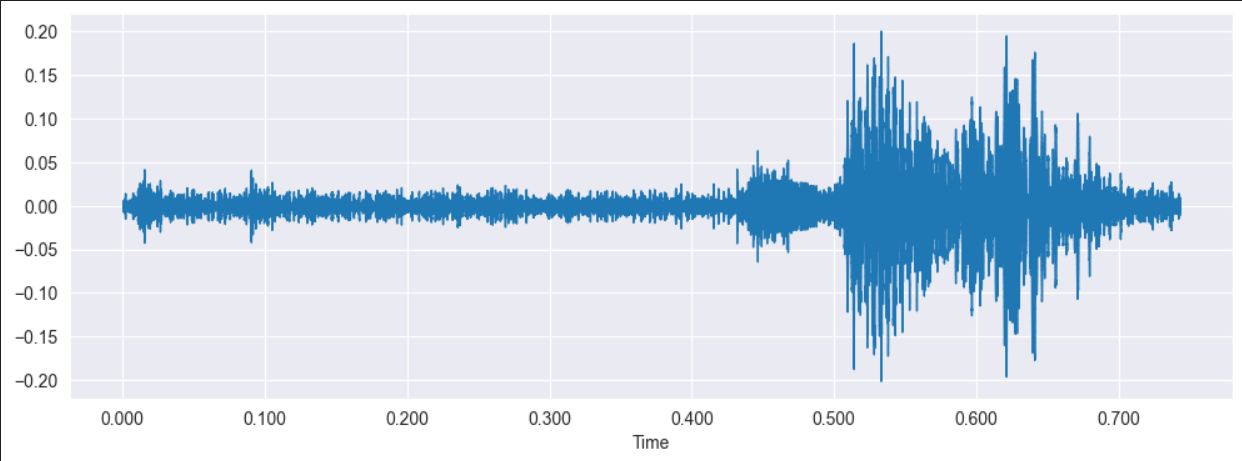
\includegraphics[width=0.5\linewidth]{spectogram.png}
    \caption{Enter Caption}
    \label{fig:enter-label}
\end{figure}
\section{Xây dựng mô hình}

\begin{figure}
    \centering
    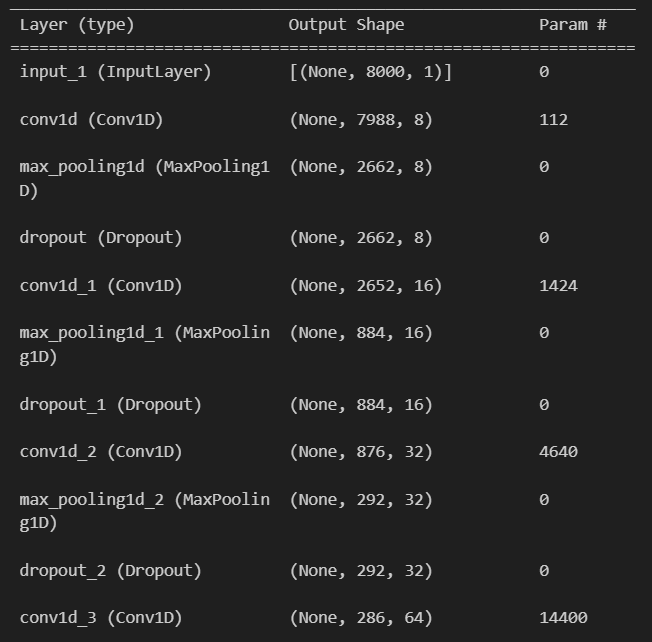
\includegraphics[width=0.5\linewidth]{images/model_1.png}
    
    
\end{figure}

\begin{figure}
    \centering
    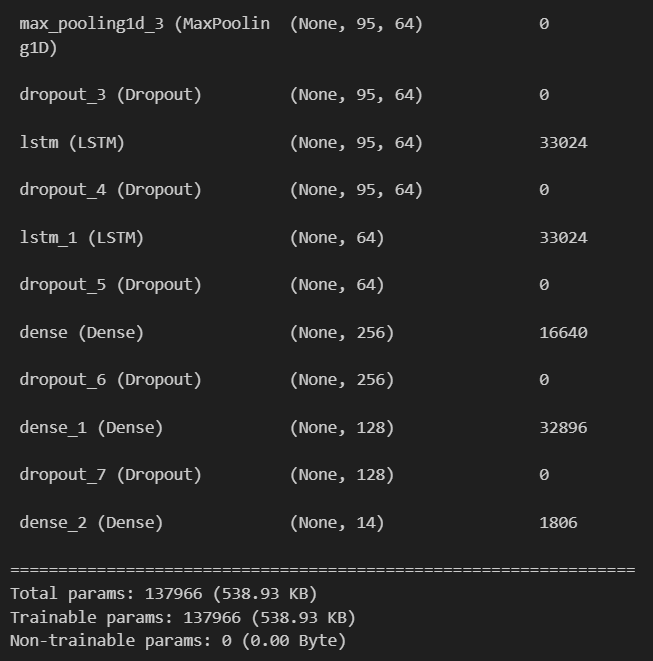
\includegraphics[width=0.5\linewidth]{images/model_2.png}
    
    
\end{figure}
\section{Đánh giá mô hình}
\begin{figure}
    \centering
    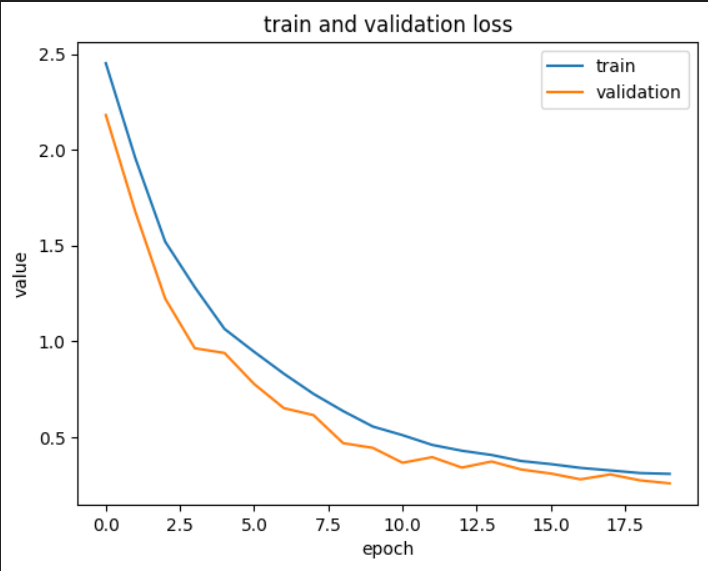
\includegraphics[width=0.5\linewidth]{images/loss.png}
    \caption{Enter Caption}
    \label{fig:enter-label}
\end{figure}

\begin{figure}
    \centering
    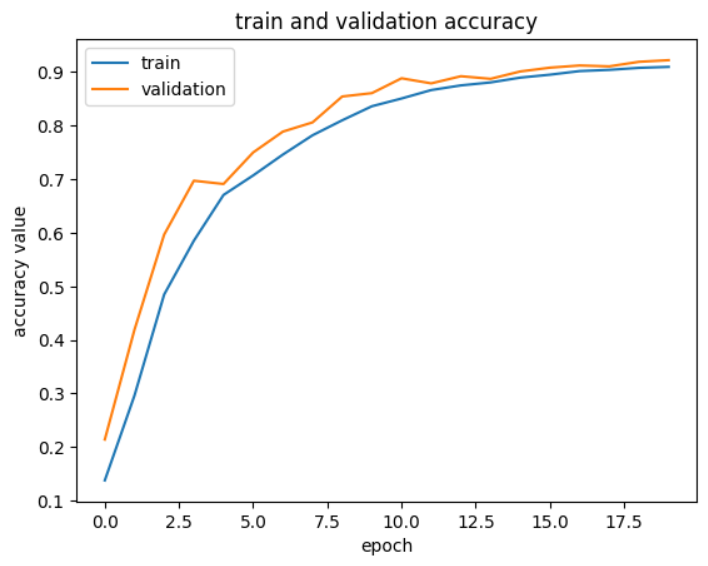
\includegraphics[width=0.5\linewidth]{images/accuracy.png}
    \caption{Enter Caption}
    \label{fig:enter-label}
\end{figure}
\begin{figure}
    \centering
    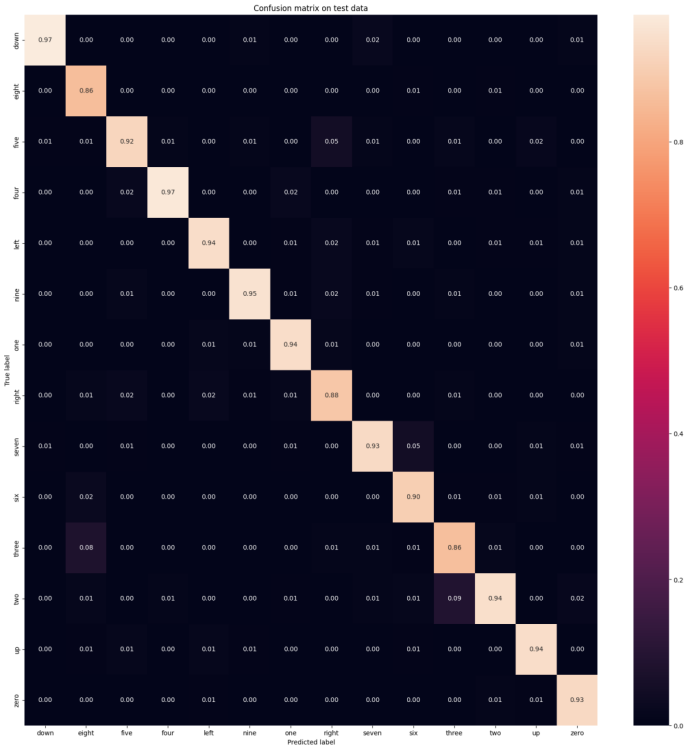
\includegraphics[width=0.5\linewidth]{images/confusion_matrix.png}
    
Accuracy: 0.9221
\end{figure}